\chapter{Results and Discussion}

In this section the models capabilities are tested and discussed. We further examine the predictions generated by the optimized neural network model and test its performance in artificially constructed as well as real-world scenarios. 

\section{Real and artificial transition regions}

While we up to this point maily have focused on leave-one-out and validation set accuracies we have not in detail studied what the classifier output looks like. We are specifically interested in examining how well performance is when the robot moves across a \emph{transition region}, a region where the surface type changes from grass to nongrass or vice versa. Ideally the prediction should rapidly change according to the new target surface. 

This can be accomplished in two different ways. The first revolves around creating a test set by concatenating the last parts of each session. By doing this, we artificially generate transition region data which we can predict on. Examining these predictions we get a feel for what output the predictor may generate when moving from one surface to the next. The second method is to simply use real-world measurements from when the robot moves across a surface. We should see that at the time point when the robot has reached the transition the prediction change accordingly. 

\begin{figure}
	\centering
	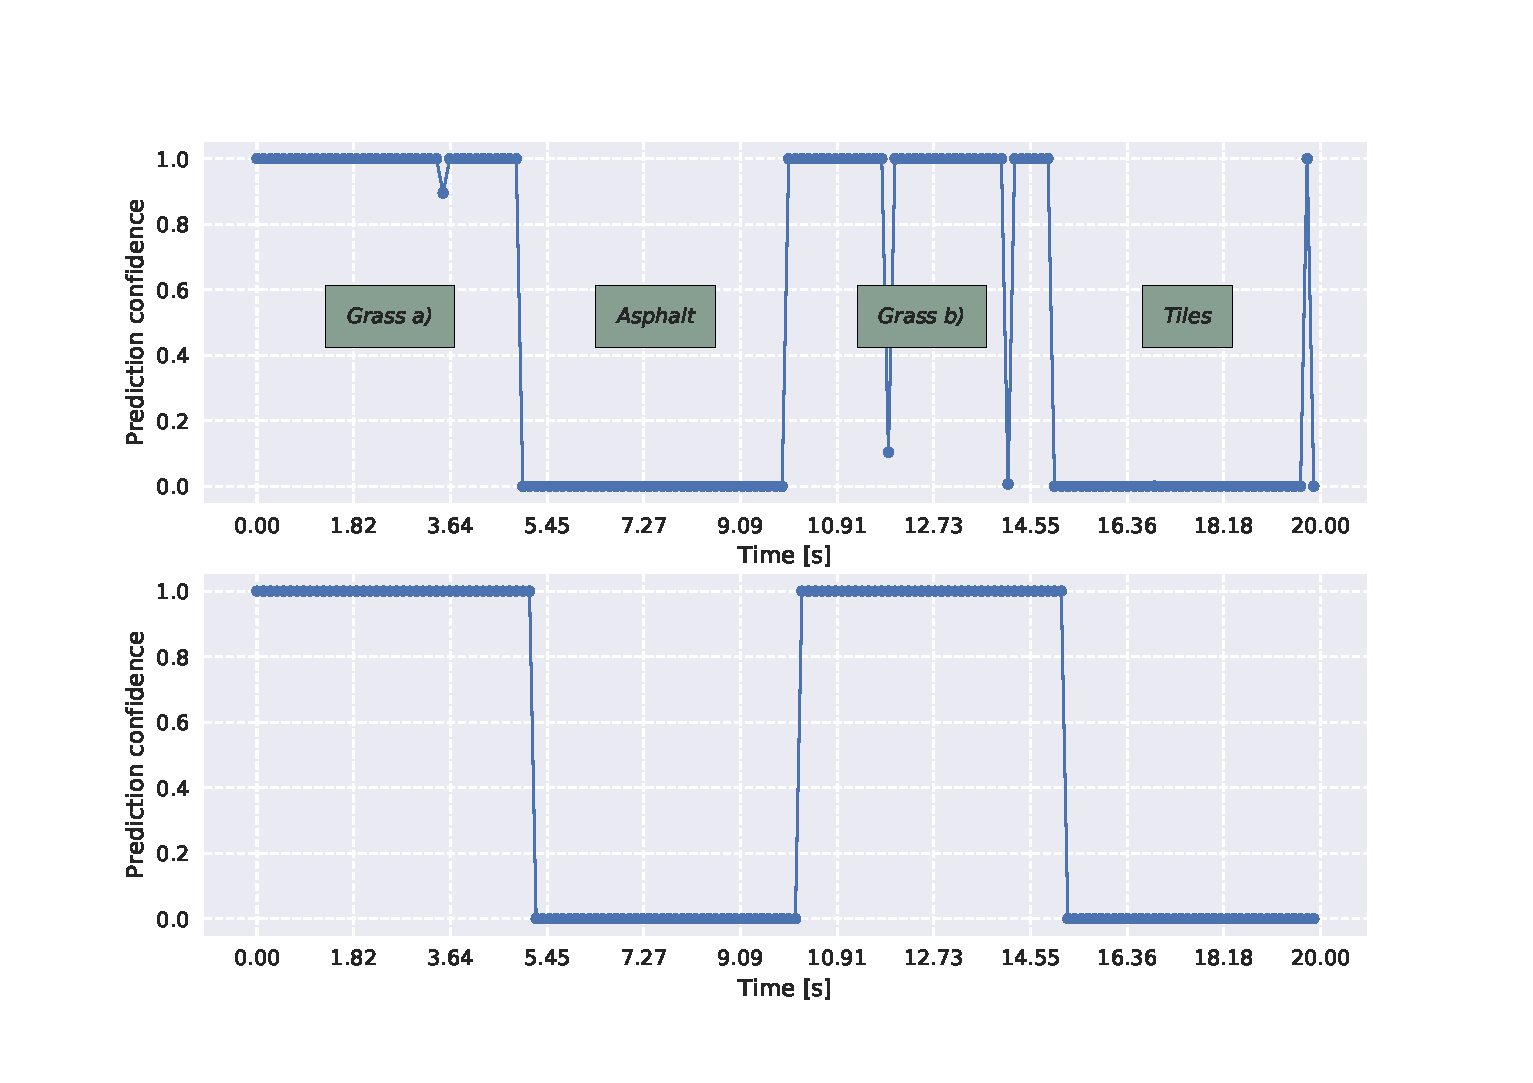
\includegraphics[scale=0.5]{figs_temp/varmats1}
	\caption{Artificial transition region created using samples from four different regions.}
\end{figure}

\begin{figure}
	\centering
	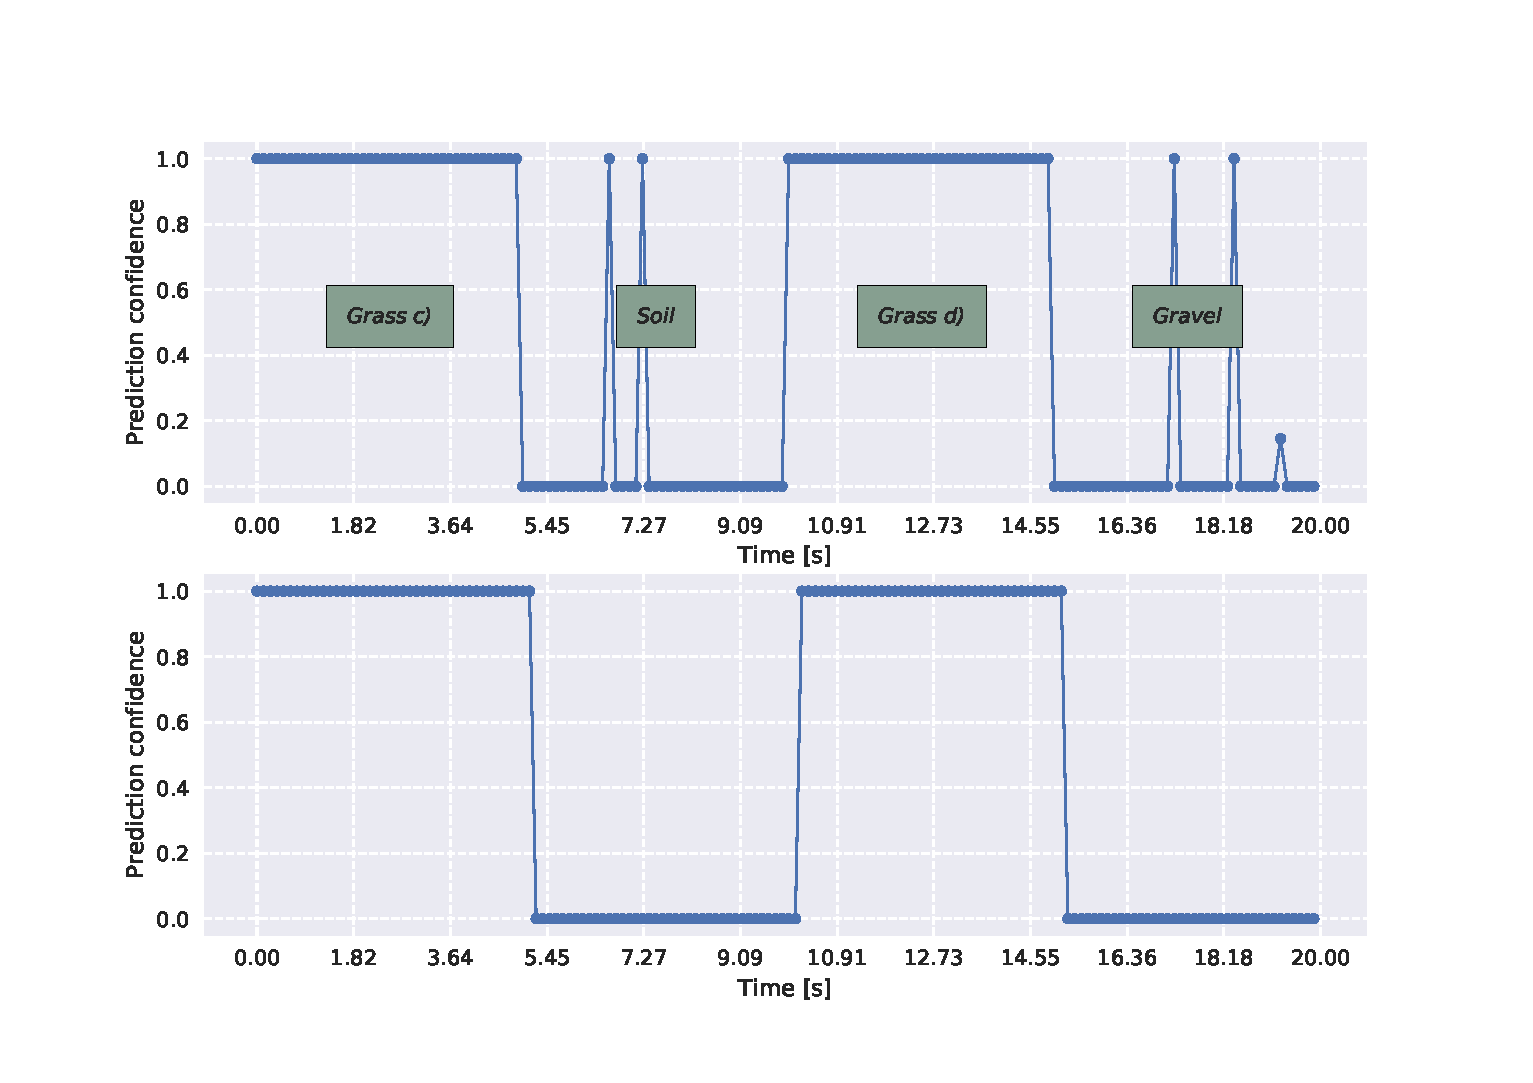
\includegraphics[scale=0.5]{figs_temp/varmats2}
	\caption{Artificial transition region created using samples from four different regions.}
\end{figure}

\begin{figure}
	\centering
	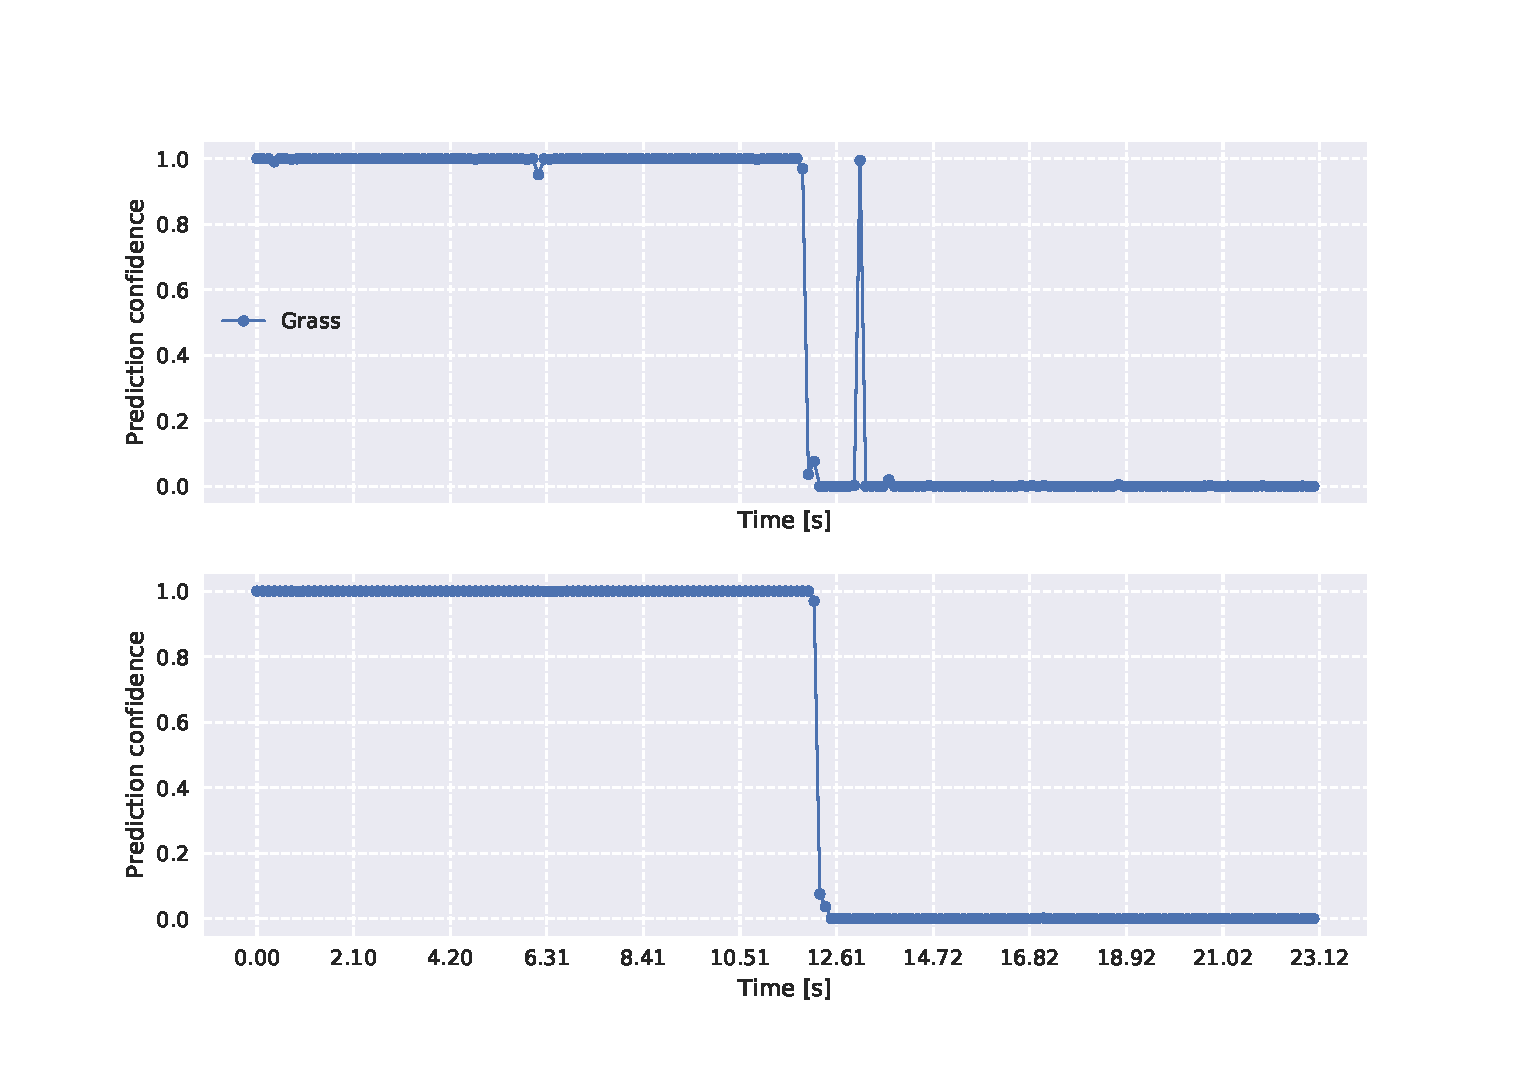
\includegraphics[scale=0.5]{figs_temp/transition_grass_tiles_grass}
	\caption{Real-world test where the robot moved across a tile pavement in a lawn.} 
	\label{fig:trans_tgtg}
\end{figure}

\begin{figure}
	\centering
	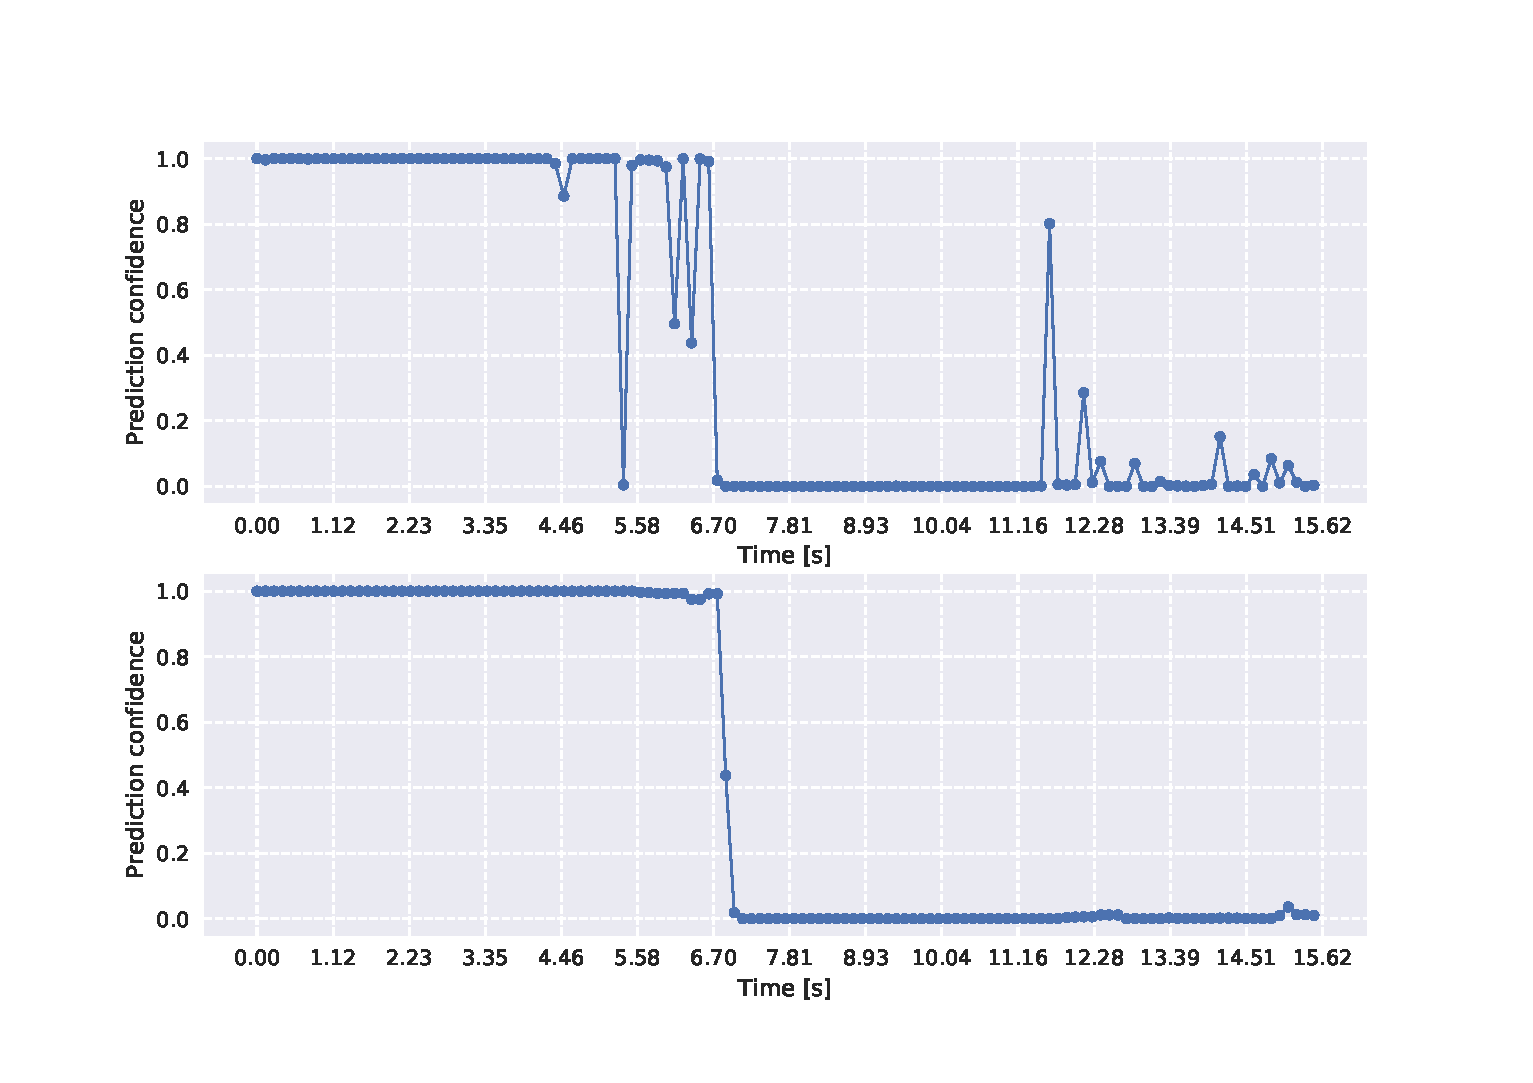
\includegraphics[scale=0.5]{figs_temp/transition_grass_gravel2}
	\caption{Real-world transition}
\end{figure}

\section{Difficult surfaces}

An often critical aspect of any machine learning system is its performance on dissimilar data: How well does the algorithn manage when we are faced with new data dissimilar to the ones seen in training? When traversing a lawn of poor quality, are we still able to classify its surface as a grassy one?  

\section{Moisture}

One particularly challenging aspect of adequately classifying surfaces is the ever-changing environmental conditions surronding the sensor. Of particular interest is the moisture content in the surfaces of interest. Greater soil moisture implies higher dielectric constant, which in turn increases radar wave scattering \citep{rappaport_2006}. Thus a single surface may very well change its scattering properties over time. 

% More things that make selecting data tricky

\section{Surface variances}

Such effects is difficult to account for when selecting data. Gather a dataset as diverse as possible

\section{Feature Extraction}
 Machine learning is used to find features it considers are good. By manually performing feat. ext. we remove information that the algorithms may otherwise have used to become even better etc. 

Future work: investigate models with no manual feat. extr.

Table [TABLENAME] is in many ways a very telling one. Here, each sample session was classified without using any of the samples from the session at hand. Instead, all other sessions were used in training. Six different methods of classification were evaluated; two linear and four nonlinear. 

First and foremost it is noted that each tested method performed at the very least \emph{decently}. One may argue that the LSTM model is unstable or that using LDA produces lower accuracy predictions, but they nonetheless generated accuracies above 97.5\%. This remarkable result means that given a random sample from the dataset collected, with no samples from the session the sample was taken from used in training, we can correcly classify the surface as grass or non-grass 39/40 times even with the lower-performing classifiers. With the top performing fully connected model, even higher accuracy was obtained with a low standard deviation. 

